\chapter{Конструкторская часть}

В данном разделе представлены схемы алгоритмов разработанного сервера для отдачи статического содержимого. Показаны алгоритмs работы процесса-предка, работы процесса-обработчика, обработки стартовой строки HTTP-запроса и формирования плана HTTP-ответа, включающего строку состояния и заголовки.

\section{Алгоритм работы процесса-предка}

На рисунке~\ref{fig:main_proc} представлена схема алгоритма работы процесса-предка.

\begin{figure}[H]
    \centering
    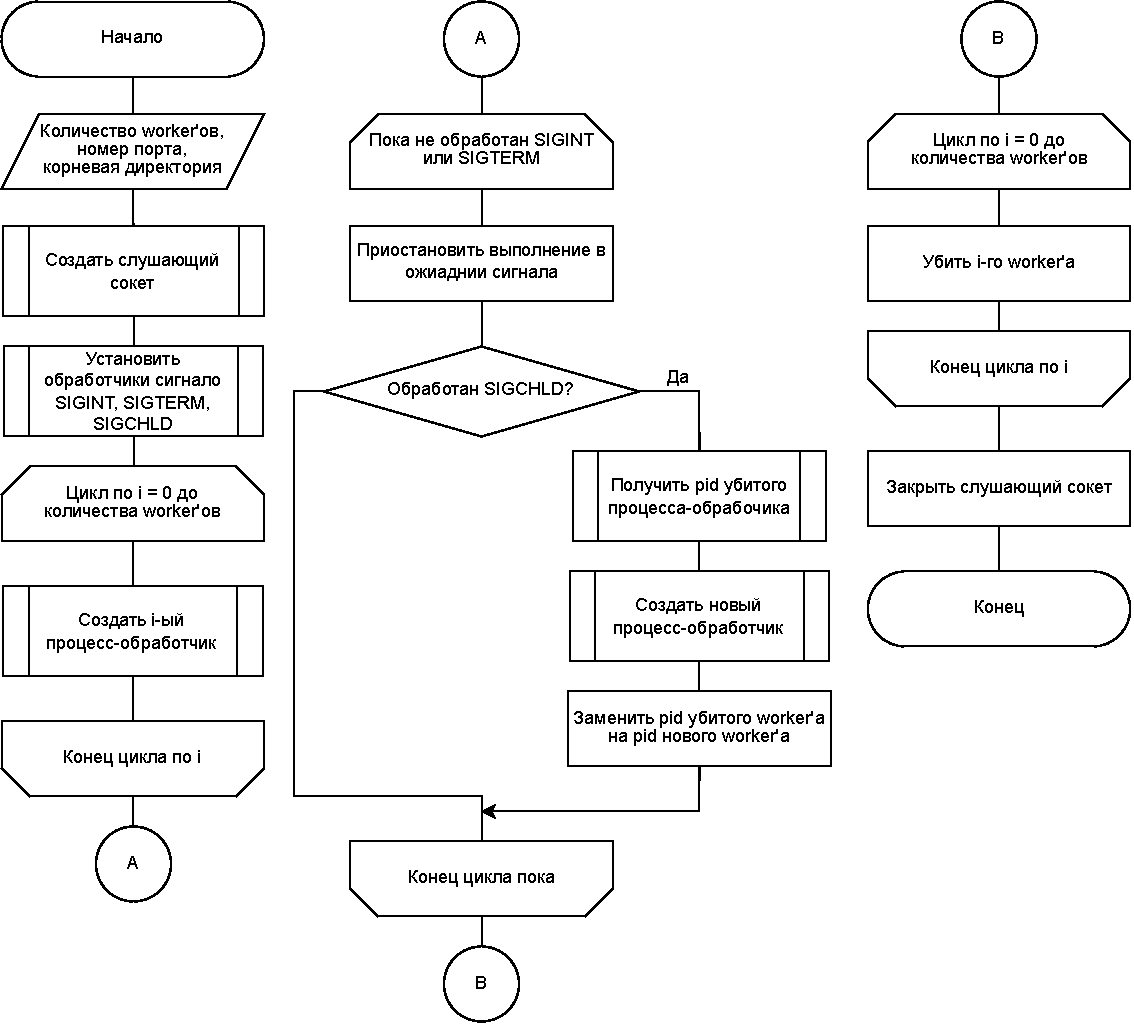
\includegraphics[width=0.95\textwidth]{images/MainScheme.pdf}
    \caption{Схема алгоритма работы процесса-предка}
    \label{fig:main_proc}
\end{figure}

На рисунке \ref{fig:worker_proc} приведена схема алгоритма работы процесса-обработчика. Процесс-обработчик ожидает запросов на соединение, принимает их, осуществляет отправку статического ресурса по частям, после полного прочтения запроса.

\begin{figure}[H]
	\centering
	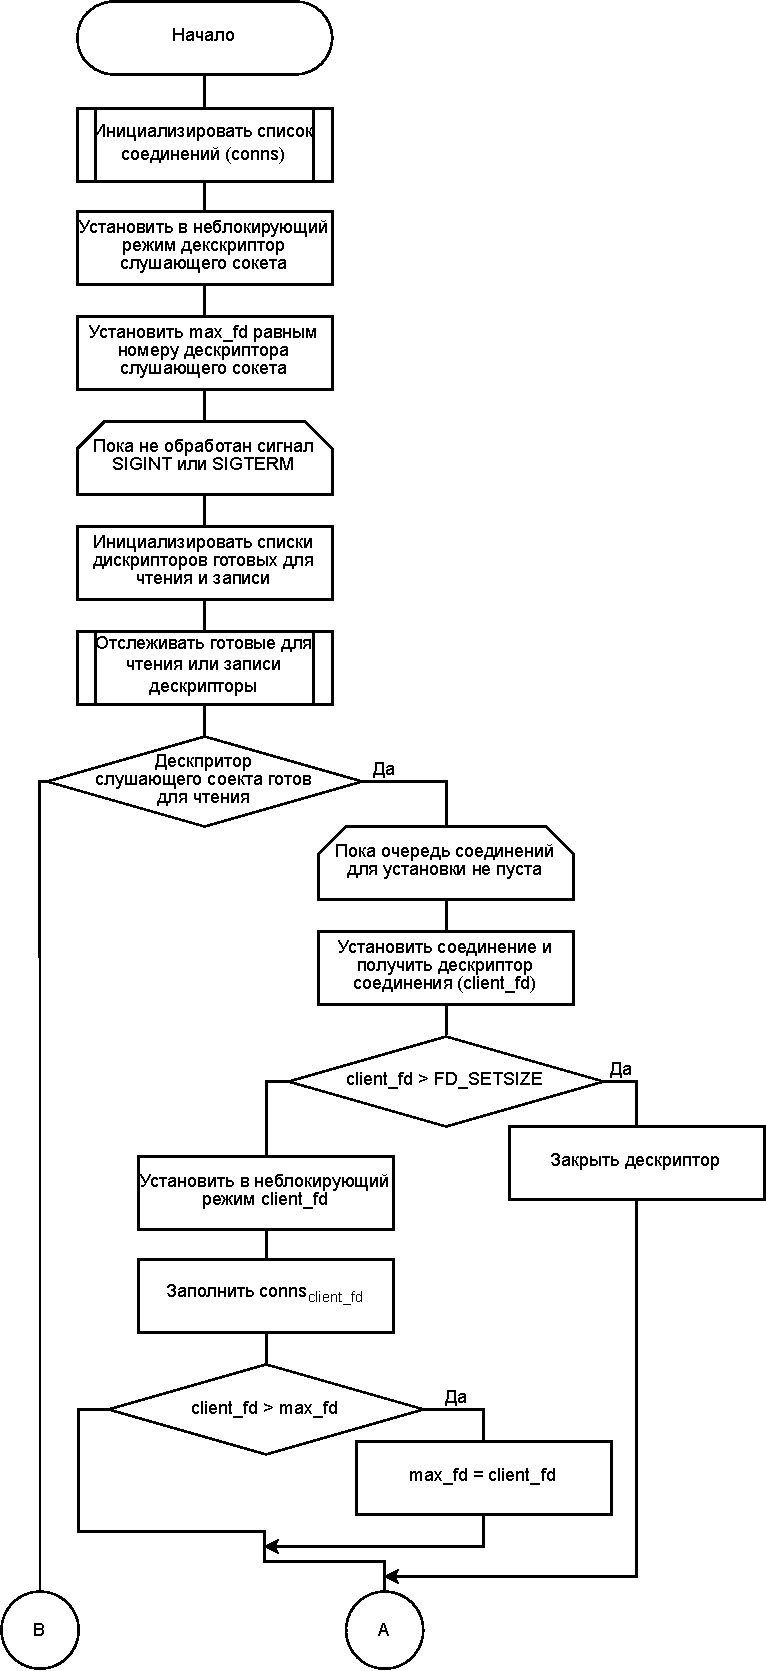
\includegraphics[height=0.95\textheight]{images/WorkerSchema1.pdf}
	\caption{Схема алгоритма работы процесса-обработчика}
	\label{fig:worker_proc}
\end{figure}
\begin{figure}[H]
	\centering
	\ContinuedFloat
	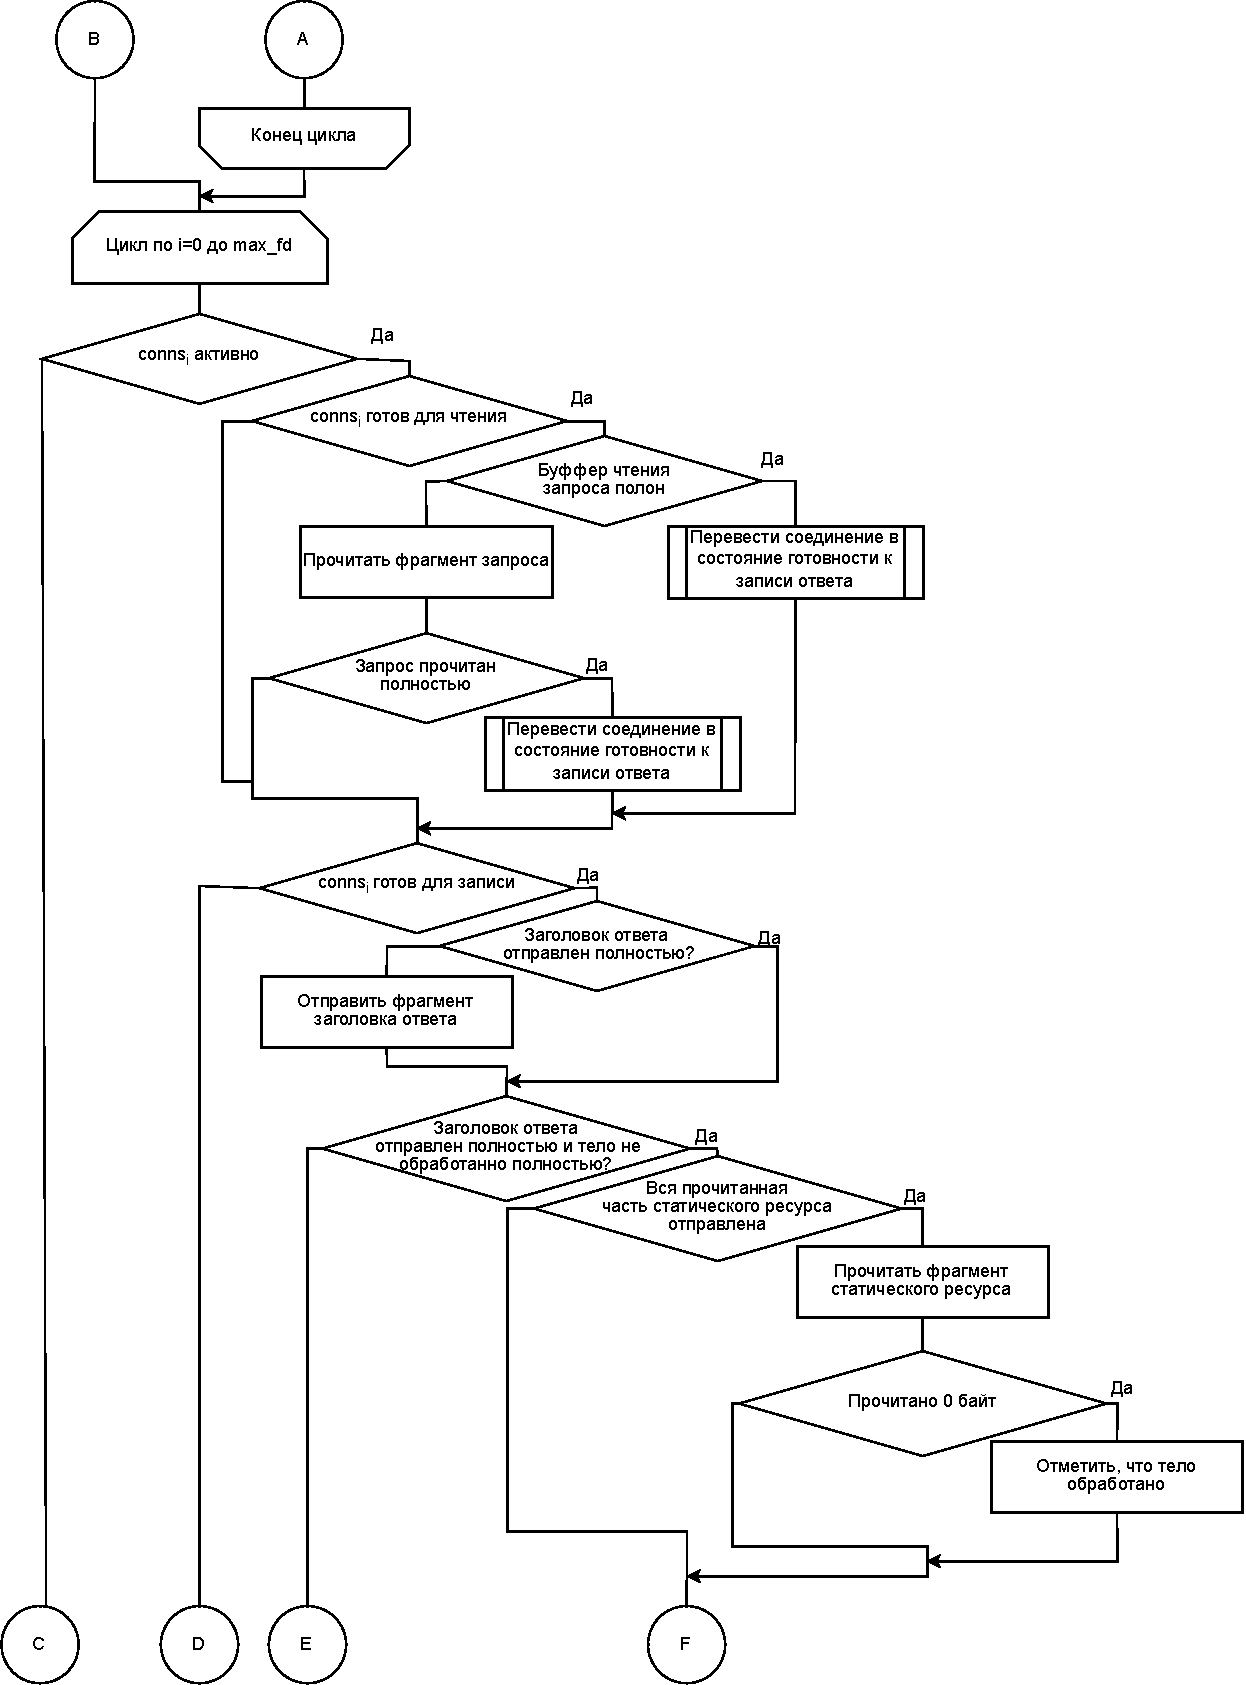
\includegraphics[width=\textwidth]{images/WorkerSchema2.pdf}
	\caption{Схема алгоритма работы процесса-обработчика}
	\label{fig:worker_proc2}
\end{figure}
\begin{figure}[H]
	\centering
	\ContinuedFloat
	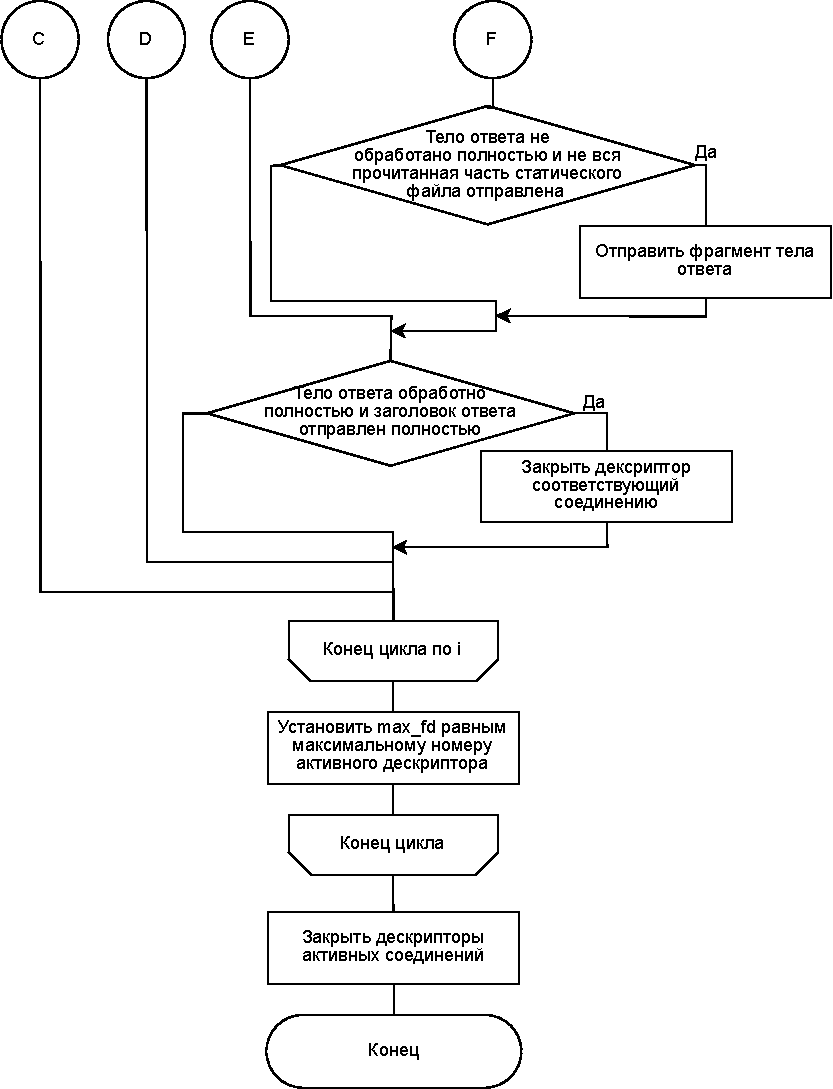
\includegraphics[width=\textwidth]{images/WorkerSchema3.pdf}
	\caption{Схема алгоритма работы процесса-обработчика}
	\label{fig:worker_proc3}
\end{figure}

На рисунке~\ref{fig:req_line_proc} представлена схема алгоритма разбора стартовой строки HTTP-запроса.

\begin{figure}[H]
	\centering
	\ContinuedFloat
	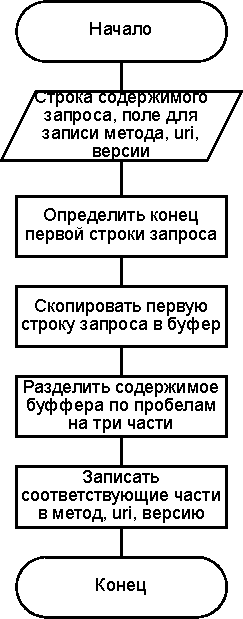
\includegraphics[height=0.4\textheight]{images/RequestLinePars.pdf}
	\caption{Схема алгоритма разбора стартовой строки HTTP-запроса}
	\label{fig:req_line_proc}
\end{figure}

На рисунке~\ref{fig:response_proc} представлена схема алгоритма формирования плана HTTP-ответа.

\begin{figure}[H]
	\centering
	\ContinuedFloat
	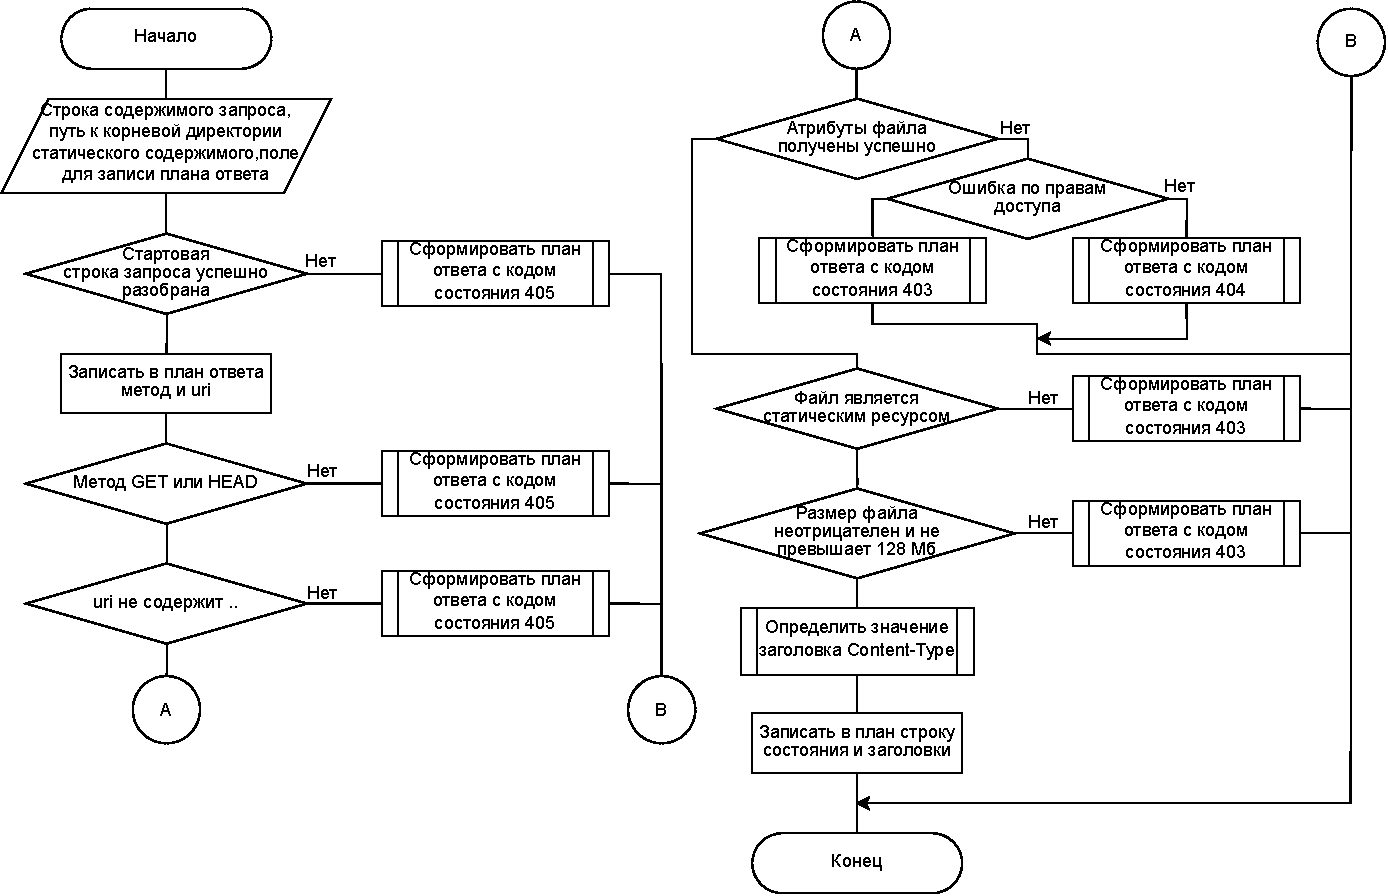
\includegraphics[width=\textwidth]{images/FormResponse.pdf}
	\caption{Схема алгоритма формирования плана HTTP-ответа}
	\label{fig:response_proc}
\end{figure}

\section*{Вывод}

В данном разделе спроектированы процедуры работы основного процесса-предка и процессов-обработчиков, а также алгоритмы разбора стартовой строки HTTP-запроса и формирования плана HTTP ответа, приведены соответствующие схемы алгоритмов.

\clearpage